% In this section, we discuss the exploration of \pred\ in the linear bandit setting discussed in \Cref{sec:short-horizon}. Recall that the linear bandit setting consist of horizon $n=25$, $\Mpr = 200000$, $\Mts = 200$, $A=10$, and $d=2$. 
% %
% %
% The demonstrator $\pi^w$ is the \ts\ algorithm and we observe that \pred\ (\gt) has lower cumulative regret than \dptg, \ad\ and matches the performance of \linucb. 
% % 
% Therefore \pred\ (\gt) behaves almost optimally in this setting and so we analyze how \pred\ conducts exploration for this setting.  
% %



% \textbf{Outcomes:} We first discuss the main outcomes of our analysis of exploration in the low-data regime:

We now state the main finding of our analysis of exploration in the linear bandit setting:

\begin{tcolorbox}
\customfinding The \pred\ (\gt) has an implicit two-phase exploration. In the first phase, it explores with a strong prior over the in-context training data. In the second phase, once the task data has been observed for a few rounds (in-context) it switches to task-based exploration.
\end{tcolorbox}

% \noindent
% \textbf{(1)} The \pred\ (\gt) has a two phase exploration. In the first phase it explores with a strong prior over the training data. In the second phase, once the task data has been observed for a few rounds it switches to task-based exploration.

% \textbf{(2)} \pred\ (\gt) samples the optimal action in each task more than \dptg. \pred (\gt) considers a larger set of possible optimal action candidate set than \dptg.




We first show in \Cref{fig:train-dist} the training distribution of the optimal actions. For each bar, the frequency indicates the number of tasks where the action (shown in the x-axis) is the optimal action.
%
Then in \Cref{fig:analysis-epxploration} we show how the sampling distribution of \dptg, \pred\, and \predt\ change in the first $10$ and last $10$ rounds for all the tasks where action $5$ is optimal. To plot this graph we first sum over the individual pulls of the action taken by each algorithm over the first $10$ and last $10$ rounds. Then we average these counts over all test tasks where action $5$ is optimal. From the figure \Cref{fig:analysis-epxploration} we see that \pred (\gt) consistently pulls the action $5$ more than \dptg. It also explores other optimal actions like $\{2,3,6,7,10\}$ but discards them quickly in favor of the optimal action $5$ in these tasks. This shows that \pred\ (\gt) only considers the optimal actions seen from the training data. Once sufficient observation have been observed for the task it switches to task-based exploration and samples the optimal action more than \dptg.

Finally, we plot the feasible action set considered by \dptg, \pred, and \predt\ in \Cref{fig:analysis-exploration-time}. To plot this graph again we consider the test tasks where the optimal action is $5$. Then we count the number of distinct actions that are taken from round $t$ up until horizon $n$. Finally we average this over all the considered tasks where the optimal action is $5$. We call this the candidate action set considered by the algorithm. From the \Cref{fig:analysis-exploration-time} we see that \dptg\ explores the least and gets stuck with few actions quickly (by round $10$). Note that the actions \dptg\ samples are sub-optimal and so it suffers a high cumulative regret (see \Cref{fig:short-horizon-lin}).  \pred\ explore slightly more than \dptg, but \predt\ explores the most. 
%
% \begin{figure}[!hbt]
% \centering
% \begin{tabular}{ccc}
% \subfigure[Train Optimal Action Distribution]{\hspace*{-0.7em}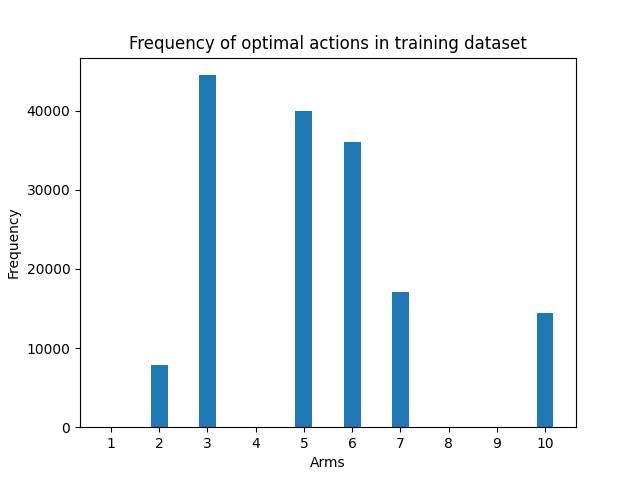
\includegraphics[scale = 0.27]{img/Neurips/linear/optimal_action_train.png}\label{fig:train-dist}} &
% %%%%%%%%%%
% \hspace*{-0.7em}\subfigure[Distribution of action sampling in all tasks where action $5$ is optimal]{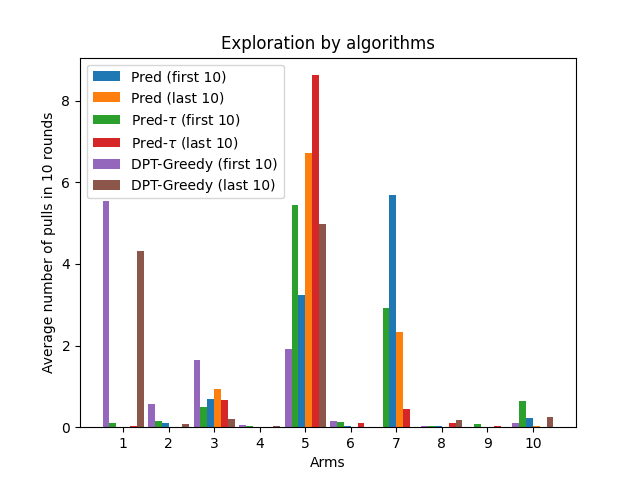
\includegraphics[scale = 0.27]{img/Neurips/linear/analysis_pull.png} \label{fig:analysis-epxploration}} &
% %%%%%%%%%%%%%%%%%%%%%%%
% \subfigure[Candidate Action Set in Time averaged over all tasks where action $5$ is optimal]{\hspace*{-0.7em}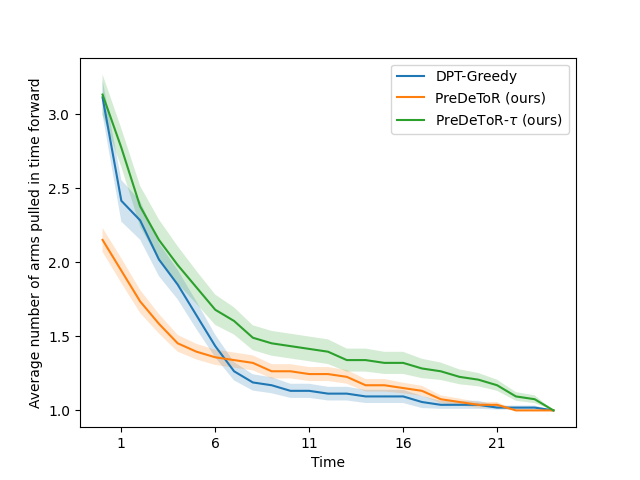
\includegraphics[scale = 0.27]{img/Neurips/linear/analysis_time_1.png}\label{fig:analysis-exploration-time}} 
% \end{tabular}
% \caption{Exploration Analysis of \pred (\gt)}
% \label{fig:exploration-analysis-time}
% \end{figure}
%
\begin{figure}[!hbt]
\vspace*{-1em}
\centering
\begin{subfigure}[b]{0.27\textwidth}
   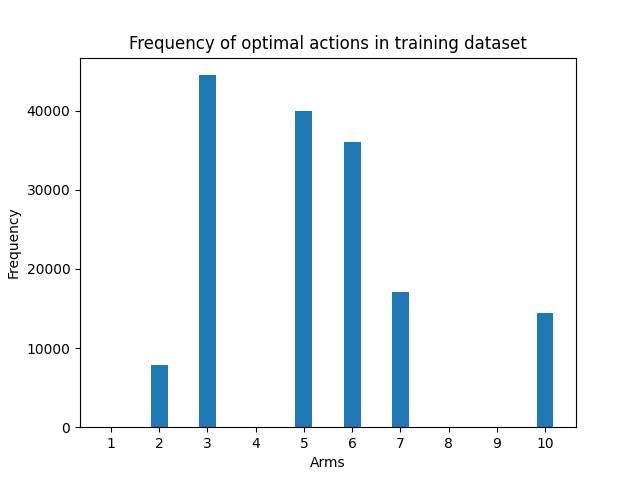
\includegraphics[scale=0.25]{img/Neurips/linear/optimal_action_train.png}
   \caption{Train Optimal Action Distribution}
   \label{fig:train-dist}
\end{subfigure}%
\hspace*{1em}\begin{subfigure}[b]{0.27\textwidth}
   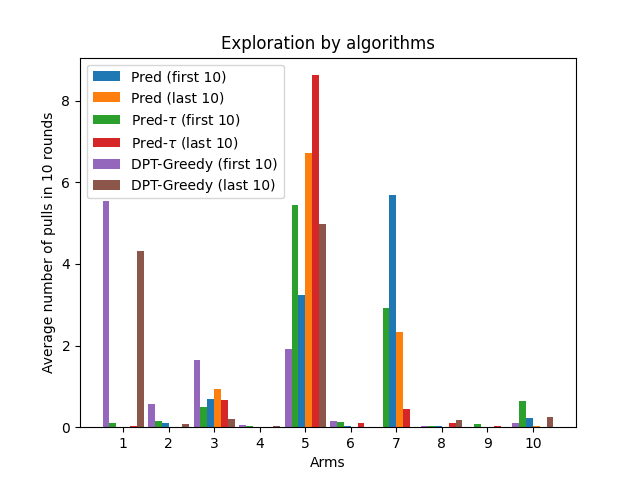
\includegraphics[scale=0.25]{img/Neurips/linear/analysis_pull.png}
   \caption{Distribution of action sampling in all test tasks where action $5$ is optimal}
   \label{fig:analysis-epxploration}
\end{subfigure}%
\hspace*{1em}\begin{subfigure}[b]{0.27\textwidth}
   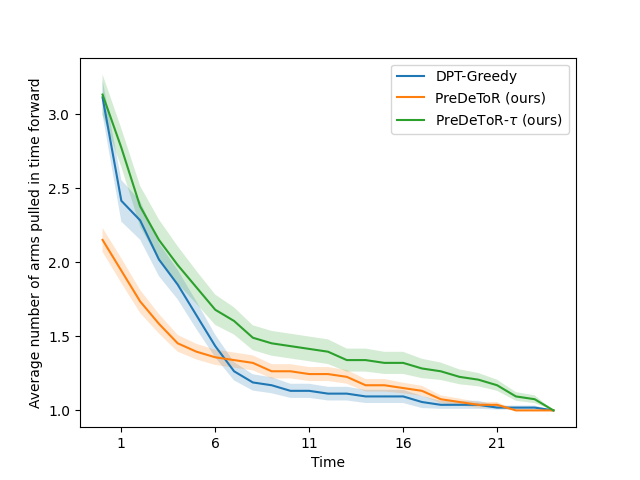
\includegraphics[scale=0.25]{img/Neurips/linear/analysis_time_1.png}
   \caption{Candidate Action Set in Time averaged over all tasks where action $5$ is optimal}
   \label{fig:analysis-exploration-time}
\end{subfigure}
\caption{Exploration Analysis of \pred (\gt)}
\label{fig:exploration-analysis-time}
\end{figure}
\vspace*{-1em}